\chapter{统计估计理论}\label{prob-stat-est}
\section{估计什么}
估计,可以是估计参数(参数估计理论),或者估计一个分布(贝叶斯分析,分类也是估计一个分布),或者估计某一个量(比如估计处理效应,这在概率论中有所分析.通常也与分布有关).

\paragraph*{估计某一个量} 给定一组样本$\{X_i\}_{i=1}^n,X_i\sim f(X_i;\theta)$,试估计$g(\theta)$。

在极大似然的框架下,可以首先通过极大似然估计$\theta$,然后直接计算$g(\theta)$。在贝叶斯框架下,需要估计的是$g(\theta;X)$,它是一个分布。

具体地说,假如是参数化模型,估计的量大致分为:
\begin{enumerate}
\item 只有确定型变量.通常就是最优化解决,如OLS.线性回归中的方差建模为确定型变量.
\item 定形随机变量.形是指形式、大小,比如线性回归中自变量的参数.可以用ML、EM估计.
\item 不定形随机变量.典型的例子是变分EM中的聚类个数.
\end{enumerate}
\section{估计中存在的问题}
各种扩展的统计模型大都是为了解决以下问题:

\begin{enumerate}
\item 噪声.当噪声为高斯时,比较好处理,非高斯就很难处理了.另外,噪声可能引起异常值,比如对一个分布进行采样,大概率会有一些值远超出平均水平,这是由概率的本性决定的.
\item 小样本.
\item 样本非独立或者非随机.我们希望样本是独立的,这样很容易拆开来分析;再者,相互作用属于非线性关系.但实践中不一定能做到随机采样,比如截断与删失(幸存者偏差也属于此类),有些样本没法观测到;又比如自相关,就是非独立.

非独立有两个维度,第一是纵向:个体间;第二是横向:变量间.潜变量模型也可以视为变量间非独立的例子.
\item 样本非同分布.只有样本本来属于同一个分布,才能通过许多样本对参数进行准确的估计,如果本来就不是同分布的,那么就难以准确地估计,因为不同样本的参数本来不一样.Mixture模型就是解决非同分布的一种方法,引入多个分布.

注意,非同分布有时不一定是一个问题,比如假如能找到驱动非同分布的变量,也可以放一起估计.从这里看,非同分布有时可能是选择的变量不完全.
\item 非线性,线性关系只有一种,而非线性关系则是无穷的.线性模型本质上相当于一阶展开式,它的一个特征时,参数在变量取不同值时的作用是一样的.
\item 分布不符合模型.通常我们是用噪声的分布指定模型的分布,所以分布不符合模型通常是说噪声分布不符合模型,比如非正态分布.
\end{enumerate}

\section{重要定义}
\subsection{估计量的性质}
\subsubsection{无偏性}
估计量的期望就是真实值:
$$\E(\hat{\btheta})=\btheta_o$$

\subsubsection{渐近一致}
$$\plim{n\rightarrow \infty} \hat{\btheta}=\btheta_o$$
实际相当于依概率收敛
\begin{equation}
\hat{\btheta}\xrightarrow{P}\btheta_o
\end{equation}

也可以表示为
$$\forall \varepsilon,\lim_{n\rightarrow \infty}\Prob\sbra{|\hat{\btheta}-\btheta_o|>\varepsilon}=0$$
另一个常见定义是样本趋于无穷大时,估计量极限为真实值,且方差为0.

注意依概率收敛弱于一致收敛:
\begin{equation}
\hat{\btheta}\xrightarrow{\text{a.s.}}\btheta_o
\end{equation}
或者
\begin{equation}
\Prob\left(\lim_{n\rightarrow \infty} \hat{\btheta}=\btheta_o\right)=1
\end{equation}
这里的意思是说概率全部集中在一点。

粗粗地看,渐近一致与无偏差不多,都描述了趋近于真实值的意思.但前者是静态的,只考虑期望,后者是动态的.一个估计量可以无偏但不渐近一致,也可以渐近一致但有偏.前者比较容易理解,只要方差没有趋于0,就没有渐近一致.

后者有点反直觉,给出一个例子:
$$\hat{\mu}=\frac{1}{N}+\frac{1}{N}\sum_{k=1}^Nx_i$$

这是有偏的,但方差是趋于0,因为常数的方差是0,加上常数不影响方差,而且样本无穷大时,前一项为0.
\subsubsection{相合估计量}

\subsubsection{无偏估计量的方差界限}
\paragraph*{Cramer Rao Bound}含义是在不同的$\theta_o$时,估计的难易程度不一样。

给定一组样本$X$,希望用它来估计$g(\theta)$,那么
$$\Var(\hat{g}(X))\geq \frac{\sdet{g'(\theta)}^2}{nI_1(\theta)}=\frac{\sdet{g'(\theta)}^2}{I(\theta)}$$
$I(\theta)$是Fisher信息矩阵\eqref{Fisher-Information},$I_1(\theta)$是单个样本的“贡献”。

如果$g(\theta)=\theta$,即直接估计$\theta$,那么有:
$$\Var(\hat{\theta})\geq \frac{1}{I(\theta)}$$

可见这个下界是与分布和参数有关的,而且注意这个下界并不总是能达到。这可以从推导过程看出来。

首先刻画无偏估计量:
\begin{empheq}{align*}
\int_x \sbra{\hat{\theta}-\theta}p(x|\theta)\dif x=0
\end{empheq}
上式中我们是用样本$x$估计参数,所以是对$x$积分。上式对$\theta$求导有:
\begin{empheq}{align*}
-\int_x p(x|\theta)\dif x+\int_x \sbra{\hat{\theta}-\theta}\frac{\partial p(x|\theta)}{\partial \theta}\dif x=0\\
\xRightarrow{} \int_x \sbra{\hat{\theta}-\theta}\frac{\partial \ln p(x|\theta)}{\partial \theta}p(x|\theta)\dif x=1
\end{empheq}
这个求导技巧在计算正态分布的方差时也使用了。

然后使用Schwaritx公式\eqref{int-Schwarz}估计方差:
$$\Var(\hat{\theta})=\int_x \sbra{\hat{\theta}-\theta}^2p(x|\theta)\dif x$$
\begin{empheq}{align*}
&\int_x\sbra{\hat{\theta}-\theta}^2p(x|\theta)\dif x \int_x \sbra{\frac{\partial \ln p(x|\theta)}{\partial \theta}}^2p(x|\theta)\dif x\\
\geq & \sbra{\int_x \sbra{\hat{\theta}-\theta}\sqrt{p(x|\theta)}\sbra{\frac{\partial \ln p(x|\theta)}{\partial \theta}}\sqrt{p(x|\theta)}\dif x}^2\\
=&1
\end{empheq}

比如对于正态分布
\begin{empheq}{align*}
I(\mu)&=nI_1(\theta)\\
&=-n\int_{\infty}^{\infty}\frac{\partial^2 \ln\phi(\frac{x-\mu}{\sigma})}{\partial^2 \mu}\phi\sbra{\frac{x-\mu}{\sigma}}\dif x\\
&=-n\int_{\infty}^{\infty}\frac{\partial^2 }{\partial^2 \mu}\sbra{-\frac{(x-\mu)^2}{2\sigma^2}}\phi\sbra{\frac{x-\mu}{\sigma}}\dif x\\
&=\frac{n}{\sigma^2}
\end{empheq}
假如$\sigma$非常小,接近0,那么只要1个样本,就基本可以确定$\mu$,反之,就很难确定。

现在用样本均值$\bar{X}$来估计$\mu$,则$\Var{\hat{\mu}}=\frac{\sigma^2}{n}$,即样本均值估计量到达了下界。

又比如,对于泊松分布,
\begin{empheq}{align*}
I(\lambda)&=-n\times \frac{1}{n}\sum_{n=0}^{\infty}\frac{\partial^2 }{\partial^2 \lambda}\sbra{C+n\ln \lambda-\lambda}p(n;\lambda)\\
&=-n\times \frac{1}{n}\sum_{n=0}^{\infty}\frac{-n }{\lambda^2}p(n;\lambda)\\
&=\frac{n}{\lambda^2}\sbra{\frac{1}{n}\sum_{n=0}^{\infty}np(n;\lambda)}\\
&=\frac{n}{\lambda}
\end{empheq}

样本均值$\bar{X}$估计量的方差是$\frac{\lambda}{n}$,也达到了下界。

对于chi-square分布
\begin{empheq}{align*}
I(\nu)&=-n\int_{\infty}^{\infty}\frac{\partial^2 \ln p(x;\nu)}{\partial^2 \nu}p(x;\nu)\dif x\\
&=-n\int_{\infty}^{\infty}\frac{\partial^2 \ln\sbra{-\ln\Gamma(\nu/2)+k\nu+C}}{\partial^2 \nu}p(x;\nu)\dif x\\
&=\frac{n}{4}\psi_1\sbra{\frac{\nu}{2}}
\end{empheq}
样本均值估计量的方差是$\frac{\nu}{n}$,它没有达到下界。


\subsection{Risk}
定义
$$\Risk(\hat{\beta})\coloneqq \E(L(\hat{\beta})-L(\beta))$$

对于LS,有
$$\Risk(\hat{\beta})=\E\|\hat{\beta}-\beta\|_\Sigma^2=\underbrace{\E\|\hat{\beta}-\bar{\beta}\|_\Sigma^2}_{\text{Variance}}+\underbrace{\|\bar{\beta}-\beta\|_\Sigma^2}_{\text{Prediction loss}}$$

其中$\Sigma=\frac{1}{n}X^TX,\|\bx\|_\Sigma=\bx^T\Sigma\bx$.
\section{估计方法概览}
\subsection{基于大数定律的估计}
估计方法大致上可以分为参数估计与非参数估计方法.参数估计预先假定一个数据的分布,并且分布完全由一组参数决定;而非参数估计不预先假定数据的分布,或者假定了分布,但分布并不由参数完全决定(比如高斯过程回归),又或者参数是无限维的.主要的非参模型有:

\begin{enumerate}
	\item 全部树方法.
	\item 核方法族.比如SVM、高斯过程回归.
	\item KNN.
\end{enumerate}

非参数模型通常与函数空间密切相关.比如给每条观测值分配一个函数,比如LOWESS,对每个点进行局部加权线性回归.


另外还有半参数方法,一部分由参数决定,另一部分不由参数决定,比如Mixture模型.

贝叶斯分析中的模型有参数模型,也有非参数模型.常见的贝叶斯回归模型均属于参数模型,比如贝叶斯线性回归.虽然贝叶斯分析把参数视为随机变量,但参数还是存在的,只不过取值是不确定的.有些贝叶斯模型的参数是无限维的,就认为它是非参数模型,比如狄利克雷回归.

所以贝叶斯分析与传统统计学的区别就是,传统统计学视参数为确定的,而贝叶斯分析视参数服从一个分布.

模型除了参数还有超参数,通常我们说的参数是指它决定了数据的分布,而超参数并不直接决定数据的分布.比如神经网络的学习率.又比如贝叶斯模型中先验分布的参数是属于超参数.

\subsection{基于小样本的估计}

\subsection{一些例子}
\subsubsection{用线性组合估计总体均值。}
\begin{example}
给定一个分布$N(\mu,1)$,现在有2个样本$X_1,X_2$。现在希望用两个样本的线性组合来估计$\mu$,即$\hat{\mu}=aX_1+bX_2$,问$a,b$在何种情况下可以得到最优的解。
\end{example}
\begin{solution}
给定$a,b$,则$\hat{\mu}$的分布是$N(a\mu+b\mu,a^2+b^2)$,此时$\mu$最有可能是$a\mu+b\mu$,立即可以得到$a+b=1$。然后此时的概率密度是$\frac{1}{\sqrt{2\pi}\sqrt{a^2+(1-a)^2}}$,最大化这个值,得到$a=b=\frac{1}{2}$。

第二种角度是从一致估计量的角度来考虑,由$\E(aX_1+bX_2)=\mu$,立即可以得到当$a+b=1$,同时计算$\Var(aX_1+bX_2)=(a^2+b^2)\Var(X)\geq \frac{1}{2}\Var(X)$,所以当$a=b=\frac{1}{2}$时,$\hat{\mu}$是方差最小的无偏估计量。

第三种角度是从极大似然考虑:$L=\phi(X_1-\hat{\mu})\phi(X_2-\hat{\mu})$,可以求出$\hat{\mu}=\frac{1}{2}(X_1+X_2)$。
	
这样其它我们得到了均值的最优估计。以上也相当于用一阶矩的最优估计。

\end{solution}
上面对于2个样本使用了极大似然估计,但实际上,只有在极少数情况下,小样本时的极大似然估计是无偏的。
\begin{example}
对于$\chi^2_v$分布,它的期望是$v$,对于2个样本,极大似然估计的情况如何?
\end{example}
\begin{solution}
在小样本时,$ML(\nu;X_1,X_2)\neq \frac{X_1+X_2}{2}$,但在大样本时
$$ML(v;X)\simeq \bar{X}$$。不仅如此,每次采样2个样本,得到$\hat{\nu_i}$的估计,重复$n$次,即便$\lim_{n\rightarrow \infty}\bar{\hat{\nu}}\neq \nu_o$,所以ML估计此时不是无偏的。

然而,即便在小样本时,样本均值仍然是$\nu$最小方差无偏线性估计量.那么对于非线性函数是否也是如此?这就是之前提到的Cramer Rao Bound,样本均值的方差没有达到下界。


\end{solution}
\section{参数估计——M估计}
M估计是一大类估计方法的统称,它通过极小化样本的某个泛函得到:

$$\sum_{k=1}^n \rho(\bm{\theta};\bm{x}_i,\bm{y}_i)$$

可以看出许多估计均属于此类.

\subsection{OLS估计}
\subsubsection{单因变量回归}
对于单一的自变量,系数为向量。OLS估计对应的泛函为

$$\rho(\bm{\theta};\bm{x}_i,y_i)=(y_i-\bm{x}_i^T\bm{\theta})^2$$

它的估计结果是:

\begin{empheq}{align*}
	\hat{\bm{\theta}}&=(X^TX)^{-1}X^T\bm{y}\\
	\Var(\hat{\bm{\theta}})&=(X^TX)^{-1}
\end{empheq}
\subsubsection{多因变量回归(向量回归)}
现在有多个因变量,则系数为一个矩阵:
$$\by=A\bx+\bm{e}$$

写成矩阵形式为:
$$Y=XA^T+E$$

注意$A$不必是一个方阵,如果取$\by_i\in\mathbb{R}^d,\bx_i\in\mathbb{R}^n$,则$A\in\mathbb{R}^{n\times d}$。仍然可以用OLS估计:
$$\rho(\bm{\theta};\bm{x}_i,\bm{y}_i)=\sum\trace\left((\bm{y}_i-\bm{x}_i^T\bm{\theta})^T(\bm{y}_i-\bm{x}_i^T\bm{\theta})\right)$$

在矩阵微分部分\ref{vector-regression-target}已经给出了上式的微分,因此可以求得
$$A=\left(\sum \by_i\bx_i^T\right)\left(\sum \bx_i\bx_i^T\right)^{-1}=Y^TX(X^TX)^{-1}$$
其中$Y_{N\times n},X_{N\times d}$.

\paragraph*{随机自变量}现在来考虑一个有意思的问题,假如$X$是一个随机生成的矩阵,即每一行为一个随机向量的值,且已知其协方差阵,问这种估计方法会得到什么。

首先$\E(X^TX)=N\Sigma_{\bm{x}}$,然后有
$$\E(A)=\bmu_{\by}\bmu_{\bx}^T\Sigma_{\bm{x}}^{-1}$$
注意到,假如两个均值向量有一个为0,则系数矩阵期望为零矩阵。于是残差矩阵为
$$E=Y-X\E(A)^T$$

\paragraph*{自变量为多向量}在向量自回归的模型,我们可能取高阶自回归项:
$$\by_i=A\by_{i-1}+B\by_{i-2}$$
其实可以把数据堆起来成为一个矩阵:
$$\by_i=\begin{bmatrix}
	A&B
\end{bmatrix}\begin{bmatrix}
\by_{i-1}\\\by_{i-2}
\end{bmatrix}$$
然后按之前的方法进行计算。

\subsubsection{加权LS}
为了解决异常值问题引入的方法.OLS中每条观测值对整体贡献是均等的,如果有异常值,就可能推高整体水平.那么一种自然的想法就是给高异常值的观测值分配一个权重.

$$\rho(\bm{\theta};\bm{x}_i,\bm{y}_i)=w_i(\bm{y}_i-\bm{x}_i^T\bm{\theta})^2$$

估计结果为:

\begin{empheq}{align*}
		\hat{\bm{\theta}}&=(X^TWX)^{-1}X^TW\bm{y}\\
		\hat{\Var(\bm{\theta})}&=(X^TWX)^{-1}
\end{empheq}

$W$是一个对角矩阵.

引入权重有许多种方式,最常见的是将$\bm{y}_i$的条件方差的倒数作为权重.这需要预先估计条件方差.一种做法是用一个另外的方程的残差方差作为条件方差,再对原方程进行估计.另一种做法是用本方程来估计条件方差并迭代改进系数(Iterated WLS).

以上是使用一组全局参数,假如对每个局部采用一小部分点进行加权回归,把各个局部拼起来形成整体,就是LOWESS回归,不过这是非参方法.神经网络的分层训练在思想上基本是一回事.
\subsection{工具变量估计}

\subsection{分位数回归}
\subsubsection{模型形式与求解}
OLS描述了变量对期望的影响,而分位数回归描述的是变量变动对分位数的影响,或者说预测值在回归线以下的比例.模型形式为

\begin{equation}\label{linear-qreg-model}
y_i^p=\alpha^p+A^p\bx_i+\epsilon_i^p
\end{equation}

$p$就表示小于$p$分位数的比例.

其距离函数是
\[
d(y,\hat{y})=\begin{cases}
(1-p)|y-\hat{y}|,&\text{ if }y\leq \hat{y}\\
p|y-\hat{y}|,&\text{ otherwise }
\end{cases}
\]

即拟合线以下的数据点权重为$(1-p)$.

整体的优化目标函数是
\begin{empheq}{align*}
\min L&=p\sum_{e_i\geq 0}|e_i|+(1-p)\sum_{e_i< 0}|e_i|\\
&=\sum_{i=0}^{n}e_i\left(pI(e_i\geq 0)+(p-1)I(e_i<0)\right)\\
&=\sum_{i=0}^n e_i(p-I(e_i<0))\\
e_i&=y_i-\hat{y}
\end{empheq}

以下展示用不同分位数进行估计得到的结果.
\begin{center}
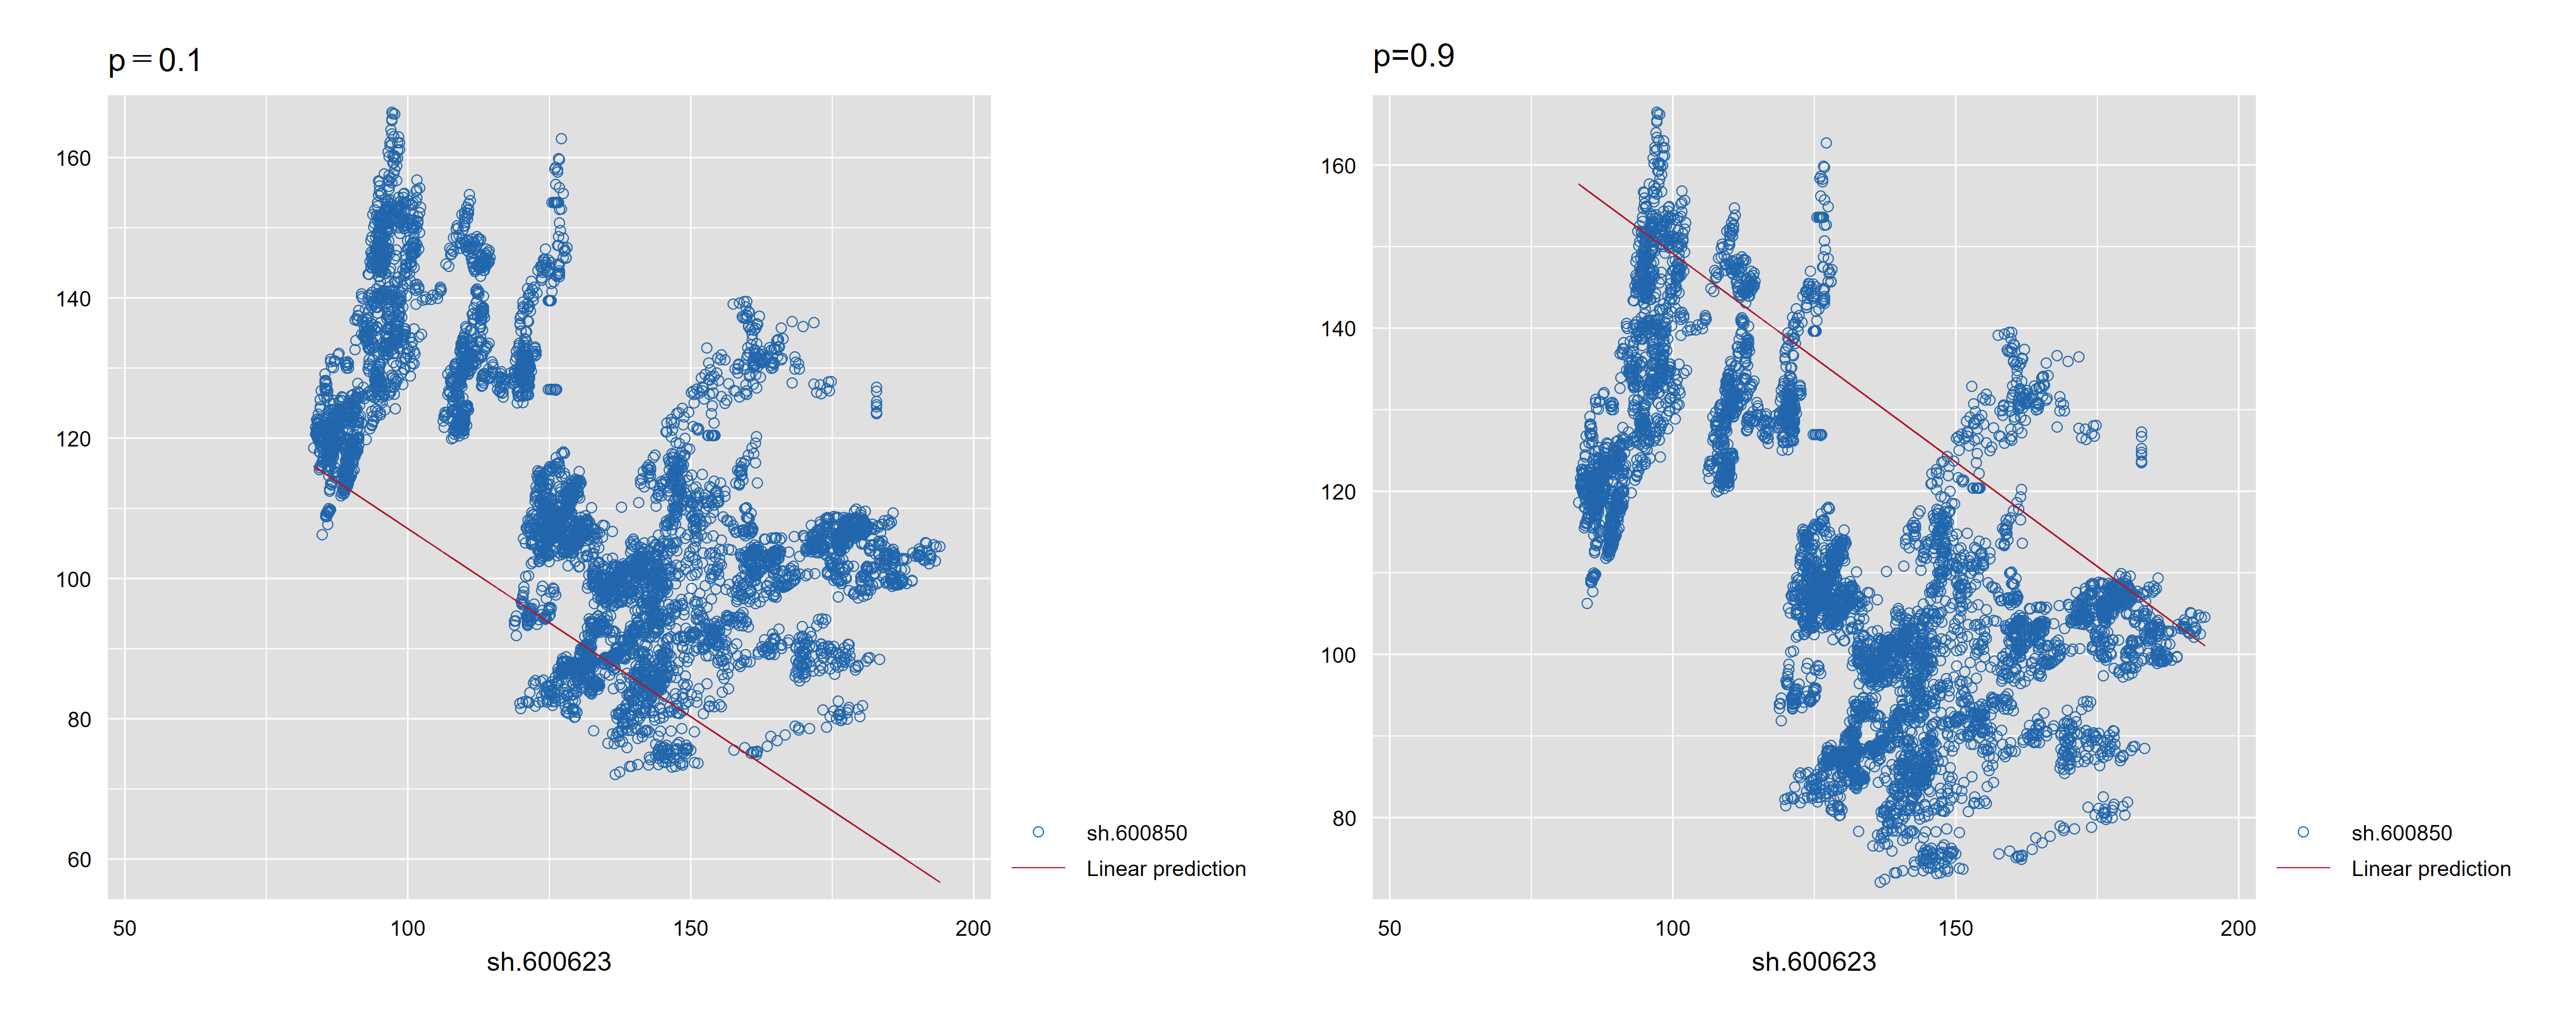
\includegraphics[width=\textwidth]{./figure/Qreg.png}
\end{center}

对于左边的图,有0.1比例的点在回归线以下,右边有0.9比例.所以分位数可以理解为
$$\E(y_i^p|\bx_i)$$

那么点在回归线以下的比例与分位数(注意每一个$\bx_i$对应一个分位数)有何关系呢?整体来看,有$p$比例的数在回归线以下,平均到每个点,就对应了每个$\bx_i$对应的分位数.反过来,$y_i^p$表示有$p$比例的$y_i$小于$y_i^p$,对应到整体就有$p$比例小于回归线.

而参数估计的置信区间就相当于进行多次分位数回归,即$y_i^{p}$的$(1-2\alpha)\%$置信区间是:
$$\left[y_i^{p_1},y_i^{p_2}\right]$$
$$p_2-p_1=1-2\alpha$$

注意这个置信区间与$p$没有直接关系.相当于说分位数的置信区间还是分位数.

由于VaR也是描述了分位数,所以一个很自然的应用就是用分位数回归计算VaR.
\subsubsection{分位数回归的优点}
\begin{enumerate}
\item 不需要假定残差的分布,适合处理非正态分布、异方差.
\item 通过对残差加权可以降低异常值的影响,另一方面,我们只看比例,那么就算异常值超出很多也关系不大,这也说明不易受异常值影响.
\item 可以设定不同的$p$拟合多条曲线.对于高斯模型,假如是异方差,则不同曲线斜率不同;同方差时,斜率是相同的.这很好理解,假如是同方差,则增大$p$时,各个$\bx_i$对应的预测值应当增加得比较均匀.

由不同的斜率可以诱导变量对不同分位数的影响,那么现实中就可以用来度量某些因素对不同收入人群的影响.
\end{enumerate}

\subsubsection{扩展}
\paragraph*{神经网络分位数回归}在\eqref{linear-qreg-model}的模型中,如果用神经网络来输出结果$\hat{y}$,就得到神经网络分位数回归。

\subsection{极大似然估计}
\subsubsection{计算}
$$\rho(\bm{\theta};\bm{x}_i,\bm{y}_i)=-\ln f(\bm{\theta};\bm{x}_i,\bm{y}_i)$$

$f$表示概率密度.

MLE估计中的一个重要度量是Fisher信息.对于单变量,定义为:
\begin{empheq}{align}
\mathcal{I}(\theta)&=E_{f(X;\theta)}\left[ \sbra{\frac{\partial \ln f(X;\theta)}{\partial \theta}}^2 \right]=-E_{f(X;\theta)}\left[\frac{\partial^2 \ln f(X;\theta)}{\partial \theta^2}\right]\mtag{Fisher Information} \label{Fisher-Information}
\end{empheq}

显然第二个等号需要函数是二次可微的,但这并不总是成立。由第一个等号可知,这个值总是大于0的。

含义是,任意无偏估计的方差不能小于这个值,所以它给出了无偏估计方差的下界.但有偏的时候,方差是可以小于这个下界的.注意,求$I(\theta)$时由于对$X$进行积分,所以并没有涉及真实的样本,而且这个值与分布和参数有关。

对于多变量,定义:
\begin{empheq}{align*}
 \mathcal{I}(\bm{\theta})&=E\left[\nabla \ln f\nabla^T \ln f|\theta\right]^2=-E\left[\textbf{H}( \ln f) | \theta\right]
\end{empheq}

\textbf{H}表示Hessian矩阵.
\subsubsection{极大似然估计的一致性}
极大似然估计是最大化:
$$\frac{1}{n}\sum_{i=1}^{N}\ln f(X_i|\theta)$$
根据大数定律,在样本无穷大时
$$\frac{1}{n}\sum_{i=1}^{N}\ln f(X_i|\theta)\rightarrow \E_{\theta_o}\ssbra{\ln f(X|\theta)}$$
最优化左边,就相当于最优化右边。右边最优化,那就是$\theta_o$。现在证明右边确实在$\theta_o$处取得最大值:
\begin{empheq}{align*}
\E_{\theta_o}\ssbra{\ln f(X|\theta)}-\E_{\theta_o}\ssbra{\ln f(X|\theta_o)}&=\E_{\theta_o}\ssbra{\ln\frac{f(X|\theta)}{f(X|\theta_o)}}\\
&\leq \ln \E_{\theta_o}\ssbra{\frac{f(X|\theta)}{f(X|\theta_o)}}\\
&=\ln \int\frac{f(x|\theta)}{f(x|\theta_o)}f(x|\theta_o)\dif x\\
&=0
\end{empheq}
当然,这个值不一定是唯一的。

\subsubsection{实例}
\paragraph*{高斯分布多元线性回归}模型为
$$\by=\bx_i^T\theta+e_i,\quad e\sim \mathcal{N}(0,\sigma^2)$$

似然函数为
$$LL(\bx_i;\btheta,\sigma^2)=\text{const}-\inv{2}\ln \sigma^2 -\frac{1}{\sigma^2}(y_i-\bx_i^T\btheta)^2$$

根据Robbins-Monro\label{Robbins-Monro}方法,导出一个Online算法:
\begin{empheq}{align}
\btheta_{i+1}&=\btheta_i+\eta (y_i-\bx_i^T\btheta_i)\bx_i=\btheta_i+\eta e_i\bx_i\label{single-var-gaussian-reg-theta}\\
\sigma_{i+1}^2&=(1-\eta)\sigma_i^2+\eta e_i^2\label{gauss-linear-reg-sigma2-online}
\end{empheq}
$\btheta_0$一般初始化为$\bm{0}$。

式\eqref{single-var-gaussian-reg-theta}中没有用到$\sigma$,可以理解为是用MSE的损失函数来推导的,如果严格按照MLE的损失函数来推导,应该是
\begin{empheq}{equation}\label{single-var-gaussian-reg-theta-no-sigma}
\btheta_{i+1}=\btheta_i+\eta \frac{e_i}{\sigma^2}\bx_i
\end{empheq}

这两个更新公式在动力学上是肯定不一样的。但最终结果却是相似的。可以这样来分析,假设初始为$\btheta^{(0)}$,用所有数据进行一次性更新(Full batch)后为$\btheta^{(1)}$。则式\cref{single-var-gaussian-reg-theta, single-var-gaussian-reg-theta-no-sigma}的更新过程分别对应为:
\begin{empheq}{align}
\btheta^{(k+1)}&=\btheta^{(k)}+\eta \sum_{i=1} (y_i-\bx_i^T\btheta^{(k)})\bx_i\\
\btheta^{(k+1)}&=\btheta^{(k)}+\eta\sum_{i=1} \frac{1}{\sigma^2}(y_i-\bx_i^T\btheta^{(k)})e_i^T\bx_i
\end{empheq}
可以理解为不动点迭代,则两式的不动点分别为:
\begin{empheq}{align}\label{single-var-gaussian-reg-theta-fixed-point}
\sum_{i=1}(y_i-\bx_i^T\btheta^{(k)})\bx_i&=0\\
\sum_{i=1}\frac{1}{\sigma^2}(y_i-\bx_i^T\btheta^{(k)})e_i^T\bx_i&=0 
\end{empheq}
显然,不动点是一样的。不过这里是假定$\sigma$为常量,实际上由于在线算法是每次用一条样本更新一次,此时不动点不再由方程\eqref{single-var-gaussian-reg-theta-fixed-point}直接给出,因此最终结果会有微小差异。

$\sigma^2$的迭代公式是这样给出的:首先计算梯度$\pdv{LL}{\sigma^2}=-\inv{2}\inv{\sigma^2}+\inv{2}e_i^2\inv{(\sigma_n^2)^2}$,直接写出的迭代公式为:
$$\sigma_{i+1}^2=\sigma_{i}^2+\eta\left(e_i^2\inv{(\sigma_i^2)^2}-\inv{\sigma_i^2}\right)$$
上式两边乘以$(\sigma_i^2)^2$有:
$$\sigma_{i+1}^2(\sigma_i^2)^2=(\sigma_i^2)^3+\eta(e_i^2-\sigma_i^2)$$
稳态时$\sigma_{i+1}^2(\sigma_i^2)^2=(\sigma_i^2)^3$,消去这两项,再在左边加上$\sigma_{i+1}^2$,右边加上$\sigma_i^2$,即可得到式\eqref{gauss-linear-reg-sigma2-online}。

\paragraph*{高斯分布向量回归}模型为
$$\by_i=A\bx_i+\bm{e}_i,\bm{e}_i\sim\mathcal{N}(\bm{0},\Sigma)$$

单样本似然函数为
$$LL(\bx_i;A,\Sigma)=-\frac{d}{2}\ln(2\pi)-\inv{2}\ln|\Sigma|-\inv{2}\bm{e}_i^T\Sigma^{-1}\bm{e}_i$$

正则方程组为
\begin{empheq}{align}
\pdv{LL}{A}&=\sum_{i=1}^{N}\Sigma^{-1}(\by_i-A\bx_i)\bx_i^T=0\\
\pdv{LL}{\Sigma^{-1}}&=\frac{N}{2}\Sigma-\inv{2}\sum_{i=1}^{N}\bm{e}_i\bm{e}_i^T=0
\end{empheq}
解为:
\begin{empheq}{align}
A&=\left(\sum_{i=1}^{N}\by_i\bx_i^T\right)\left(\sum_{i=1}^{N}\bx_i\bx_i^T\right)^{-1}=Y^TX(X^TX)^{-1}\\
\Sigma&=\inv{N}\sum_{i=1}^{N}\bm{e}_i\bm{e}_i^T=\inv{N}(Y-XA^T)^T(Y-XA^T)
\end{empheq}
式中$Y\in \mathbb{R}^{n\times d}$,为将$\by_i^T$按行堆积后形成的矩阵。同样的结果用OLS估计也可以得到。

同时导出Robbins-Monro类Online算法:
\begin{empheq}{align}
A_{i+1}&=A_i+\eta \bm{e}_i\bx_i^T \label{mv-gaussian-reg-A}\\
\Sigma_{i+1}&=(1-\eta)\Sigma_i+\eta \bm{e}_i\bm{e}_i^T\\
\Sigma_{i+1}^{-1}&=\Sigma_{i}^{-1}+\eta (\Sigma_i-\bm{e}_i\bm{e}_i^T)
\end{empheq}

\paragraph*{t分布多元线性回归}形式与高斯多元线性回归相同,只是分布假设不一样,由于t分布的长尾特性,适合进行Robust回归。
$$y_i=\bx_i^T\theta+e_i,\quad e\sim t_{\nu}(0,\sigma^2)$$
$\nu$一般可以固定为3,作为参数来学习也是可以的。

对数似然函数为
$$LL=\ln\Gamma\left(\frac{\nu+1}{2}\right)-\ln\Gamma\left(\frac{\nu}{2}\right)-\inv{2}\ln(\nu\pi)-\inv{2}\ln\sigma^2-\frac{\nu+1}{2}\ln\left(1+\inv{\nu}\left(\frac{(y_i-\bx_i^T\btheta)^2}{\sigma^2}\right)\right)$$

首先求出梯度:
\begin{empheq}{align*}
\alpha_i&=\frac{\nu+1}{\nu+e_i^2/\sigma^2}\\
\pdv{LL}{\btheta}&=\alpha_i\inv{\sigma^2}e_i\bx_i\\
\pdv{LL}{\sigma^2}&=\inv{2}\left(-\inv{\sigma^2}+\alpha_i\frac{e_i^2}{(\sigma^2)^2}\right)\\
\pdv{LL}{\nu}&=\inv{2}\left(\psi\left(\frac{\nu+1}{2}\right)-\psi\left(\frac{\nu}{2}\right)-\inv{\nu}-\ln\left(1+\inv{\nu}\left(\frac{e_i^2}{\sigma^2}\right)\right)+\alpha_i\frac{e_i^2}{\sigma^2}\inv{\nu}\right)
\end{empheq}
上式中$\psi(x)$为特殊函数\ref{digamma}。从以上也可以看出t分布回归与高斯分布回归的关系,当$\nu\rightarrow\infty$时,$\alpha_i\rightarrow 1$,则更新过程趋于高斯分布回归。

$\btheta,\nu$的更新公式立即可得,不过$\sigma^2$的更新公式可以进行一下变换:
\begin{empheq}{align*}
\sigma_{n+1}^2&=\sigma_n^2+\eta \frac{e_i^2-\sigma^2}{e_i^2+\nu\sigma^2}
\end{empheq}

另一方面可以重参数化,更新$\inv{\sigma^2}$,导数为:
$$\pdv{LL}{(\sigma^2)^{-1}}=\inv{2}\sigma^2-\inv{2}\frac{\nu+1}{\nu+e_i^2(\sigma^2)^{-1}}e_i^2$$
得到更新公式为:
$$\sigma_{n+1}^{-2}=\sigma_{n}^{-2}+\eta\left(1/\sigma_{n}^{-2}-\alpha_ie_i^2\right)$$

由于t分布的长尾特性,可以猜测使用$t$分布回归得到的$\sigma^2_{\text{t}}<\sigma^2_{\text{Gaussian}}$,因为前者会“忽略”一些异常值。

\paragraph*{t分布向量线性回归}模型为
$$\by_i=A\bx_i+\bm{e}_i,\bm{e}_i\sim t_{\nu}(\bm{0},\Sigma),A\in\mathbb{R}^{d\times k},\bx_i\in\mathbb{R}^d,\by\in\mathbb{R}^n$$

对数似然函数为:
\begin{empheq}{align}
LL(\bx_i;A,\nu,\Sigma)=\ln\Gamma\left(\frac{\nu+d}{2}\right)-\ln\Gamma\left(\frac{\nu}{2}\right)-\frac{d}{2}\ln(\nu\pi)-\inv{2}\ln|\Sigma|-\frac{\nu+d}{2}\ln\left(1+\inv{\nu}\bm{e}_i^T\Sigma^{-1}\bm{e}_i\right)
\end{empheq}

导数为:
\begin{empheq}{align}
\alpha_i&=\frac{\nu+d}{\nu+\bm{e}_i^T\Sigma^{-1}\bm{e}_i}\\
\pdv{LL}{A}&=\alpha_i\Sigma^{-1}\bm{e}_i\bx_i^T\\
\pdv{LL}{\Sigma}&=\inv{2}(-\Sigma^{-1}+\alpha(\Sigma^{-1}\bm{e})(\Sigma^{-1}\bm{e})^T)=\inv{2}(-\Sigma^{-1}+\alpha\Sigma^{-1}(\bm{e}\bm{e})^T\Sigma^{-1})\\
\pdv{LL}{\Sigma^{-1}}&=\inv{2}\left(\Sigma-\alpha\bm{e}_i\bm{e}_i^T\right)\\
\pdv{LL}{\nu}&=\inv{2}\left(\psi\left(\frac{\nu+d}{2}\right)-\psi\left(\frac{\nu}{2}\right)-\frac{d}{\nu}-\ln\left(1+\inv{\nu}\bm{e}_i^T\Sigma^{-1}\bm{e}_i\right)+\alpha_i \frac{\bm{e}_i^T\Sigma^{-1}\bm{e}_i}{\nu}\right)
\end{empheq}

实践中看,如果使用在线算法,那更新$\Sigma,\Sigma^{-1}$效果差别不明显,不过后者的复杂度稍低,收敛速度稍快。此外如果更新$\Sigma^{-1}$,那么$\det$那一项应该是$+\inv{2}\ln|\Sigma^{-1}|$,不要搞错前面的符号。步长要足够小,大概$10^{-3}$不错。
\subsection{矩估计}

\section{参数估计——贝叶斯估计}
\subsection{后验分布的计算}
\subsubsection{线性回归}
线性回归$\by=X\btheta+\bmeta,\btheta\sim \mathcal{N}(\bmu_{\btheta},\Sigma_{\btheta}),\btheta\in\mathbb{R}^{k\times 1},\bmeta\in\mathbb{R}^{n\times 1}$,注意,一般的线性回归中是假设$\btheta$不为随机变量。则分布
\begin{empheq}{align}
p(\btheta)&=\mathcal{N}\sbra{\btheta-\bmu_{\btheta},\Sigma_{\btheta}}\\
p(\by)&=\mathcal{N}(\by-X\bmu_{\btheta},\Sigma_{\bmeta}+X\Sigma_{\btheta}X^T)\\
p(\by|\btheta)&=\mathcal{N}(\by-X\btheta,\Sigma_{\bmeta})
\end{empheq}
后验分布
\begin{empheq}{align}\label{linear-gauss-posterior}
p(\btheta|\by)&=\mathcal{N}(\btheta-\bmu_{\btheta|\by},\Sigma_{\btheta|\by})\\
\bmu_{\btheta|\by}&=\bmu_{\btheta}+\left(\Sigma_{\btheta}^{-1}+X^T\Sigma_{\bmeta}^{-1}X\right)^{-1}X^T\Sigma_{\bmeta}^{-1}(\by-X\bmu_{\btheta})\\
\Sigma_{\btheta|\by}&=\left(\Sigma_{\btheta}^{-1}+X^T\Sigma_{\bmeta}^{-1}X\right)^{-1}
\end{empheq}

这个后验分布非常难算,最直接的办法就是用贝叶斯公式强行计算:
\begin{empheq}{align*}
p(\btheta|\by)&=\frac{p(\by|\btheta)p(\btheta)}{p(\by)}\\
\end{empheq}
完整展开如下:
\begin{empheq}{align*}
&(2\pi)^{-\frac{n}{2}}\left|\Sigma_{\bmeta}\right|^{-\frac{1}{2}}\exp\left(-\frac{1}{2}(\by-X\btheta)^T\Sigma_{\bmeta}^{-1}(\by-X\btheta)\right)\\
\times & (2\pi)^{-\frac{k}{2}}\left|\Sigma_{\btheta}\right|^{-\frac{1}{2}}\exp\left(-\frac{1}{2}\sbra{\btheta-\bmu_{\btheta}}^T\Sigma_{\btheta}^{-1}\sbra{\btheta-\bmu_{\btheta}}\right)\\
\hline &(2\pi)^{-\frac{n}{2}}\left|\Sigma_{\bmeta}+X\Sigma_{\btheta}X^T\right|^{-\frac{1}{2}}\exp\left(-\frac{1}{2}(y-X\bmu_{\btheta})^T\left(\Sigma_{\bmeta}+X\Sigma_{\btheta}X^T\right)^{-1}(y-X\bmu_{\btheta})\right)
\end{empheq}
可以看出这个后验分布显然还是高斯分布,因为指数项是二次的。上式中常数项可以约掉$n$的指数。然后考虑$\det$项。
\begin{empheq}{align*}
\frac{\left|\Sigma_{\bmeta}\right|^{-\frac{1}{2}}\left|\Sigma_{\btheta}\right|^{-\frac{1}{2}}}{\left|\Sigma_{\bmeta}+X\Sigma_{\btheta}X^T\right|^{-\frac{1}{2}}}&=\left|\Sigma_{\btheta}\right|^{-\frac{1}{2}}\left|\Sigma_{\bmeta}\left(\Sigma_{\bmeta}+X\Sigma_{\btheta}X^T\right)^{-1}\right|^{-\frac{1}{2}}\\
&=\left|\Sigma_{\btheta}\right|^{-\frac{1}{2}}\left|\left(I_n+\Sigma_{\bmeta}^{-1}X\Sigma_{\btheta}X^T\right)^{-1}\right|^{-\frac{1}{2}}\\
\underline{\sdet{I_n+AB^T}=\sdet{I_k+A^TB}}&=\left|\Sigma_{\btheta}\right|^{-\frac{1}{2}}\sdet{\left(I_k+X^T\Sigma_{\bmeta}^{-1}X\Sigma_{\btheta}\right)^{-1}}^{-\frac{1}{2}}\\
\underline{\sdet{A^{-1}+A^{-1}BA}=\sdet{A^{-1}+B}}&=\sdet{\sbra{\Sigma_{\btheta}^{-1}+\Sigma_{\btheta}^{-1}X^T\Sigma_{\bmeta}^{-1}X\Sigma_{\btheta}}^{-1}}^{-\frac{1}{2}}\\
&=\sdet{\sbra{\Sigma_{\btheta}^{-1}+X^T\Sigma_{\bmeta}^{-1}X}^{-1}}^{-\frac{1}{2}}
\end{empheq}

其实这里已经求出了条件分布的协方差阵。现在来考虑指数项,省略前面的$-\frac{1}{2}$:
\begin{empheq}{align*}
&\sbra{\by-X\btheta}^T\Sigma_{\bmeta}^{-1}\sbra{\by-X\btheta}+\sbra{\btheta-\bmu_{\btheta}}^T\Sigma_{\btheta}^{-1}\sbra{\btheta-\bmu_{\btheta}}-(y-X\bmu_{\btheta})^T\left(\Sigma_{\bmeta}+X\Sigma_{\btheta}X^T\right)^{-1}(y-X\bmu_{\btheta})\\
=&\sbra{\by-X\btheta}^T\Sigma_{\bmeta}^{-1}\sbra{\by-X\btheta}+\sbra{\btheta-\bmu_{\btheta}}^T\Sigma_{\btheta}^{-1}\sbra{\btheta-\bmu_{\btheta}}\\
&-(y-X\bmu_{\btheta})^T\left(\Sigma_{\bmeta}^{-1}-\Sigma_{\bmeta}^{-1}X\left(\Sigma_{\btheta}^{-1}+X^T\Sigma_{\bmeta}^{-1}X\right)^{-1}X^T\Sigma_{\bmeta}^{-1}\right)^{-1}(y-X\bmu_{\btheta})\\
=&\sbra{\by-X\btheta}^T\Sigma_{\bmeta}^{-1}\sbra{\by-X\btheta}+\sbra{\btheta-\bmu_{\btheta}}^T\Sigma_{\btheta}^{-1}\sbra{\btheta-\bmu_{\btheta}}-(y-X\bmu_{\btheta})^T\Sigma_{\bmeta}^{-1}(y-X\bmu_{\btheta})\\
&+\uwave{(y-X\bmu_{\btheta})^T\Sigma_{\bmeta}^{-1}X\sbra{\Sigma_{\btheta}^{-1}+X^T\Sigma_{\bmeta}^{-1}X}^{-1}}\underline{\sbra{\Sigma_{\btheta}^{-1}+X^T\Sigma_{\bmeta}^{-1}X}}\uwave{\sbra{\Sigma_{\btheta}^{-1}+X^T\Sigma_{\bmeta}^{-1}X}^{-1}X^T\Sigma_{\bmeta}^{-1}(y-X\bmu_{\btheta})}
\end{empheq}

上式的第二部分是显面易见的二次型,现在只需要考虑第一部分。基本思路是把第一部分的第一项拆开,再与第三项组合,第一部分
\begin{empheq}{align*}
&\sbra{y-X\bmu_{\btheta}+X\bmu_{\btheta}-X\btheta}^T\Sigma_{\bmeta}^{-1}\sbra{y-X\bmu_{\btheta}+X\bmu_{\btheta}-X\btheta}+\sbra{\bmu_{\btheta}-\btheta}^T\Sigma_{\btheta}^{-1}\sbra{\bmu_{\btheta}-\btheta}-(y-X\bmu_{\btheta})^T\Sigma_{\bmeta}^{-1}(y-X\bmu_{\btheta})\\
=&\sbra{\bmu_{\btheta}-\btheta}^T\underline{\sbra{\Sigma_{\btheta}^{-1}+X^T\Sigma_{\bmeta}^{-1}X}}\sbra{\bmu_{\btheta}-\btheta}+2\sbra{y-X\bmu_{\btheta}}^T\Sigma_{\bmeta}^{-1}X(\bmu_{\btheta}-\btheta)\\
=&\sbra{\bmu_{\btheta}-\btheta}^T\underline{\sbra{\Sigma_{\btheta}^{-1}+X^T\Sigma_{\bmeta}^{-1}X}}\sbra{\bmu_{\btheta}-\btheta}\\
&+2\uwave{\sbra{y-X\bmu_{\btheta}}^T\Sigma_{\bmeta}^{-1}X\sbra{\Sigma_{\btheta}^{-1}+X^T\Sigma_{\bmeta}^{-1}X}^{-1}}\underline{\sbra{\Sigma_{\btheta}^{-1}+X^T\Sigma_{\bmeta}^{-1}X}}\sbra{\bmu_{\btheta}-\btheta}
\end{empheq}
再与原来的第二部分合并起来看,二次型已经非常明显了。

\section{随机逼近理论}
\subsection{Robbins-Monro方法}\label{Robbins-Monro}
假设我们希望求解
$$f(\btheta)=\E(\phi(\btheta,\bbeta))$$
的零点,其中$\eta$为未知的统计量,假设它是已知的,则可以用一般的解方程组方法求解。在未知的情况下,$f$的具体形式是不知道的。Robbins-Monro方法就是给定一组独立同分布的观测值$\bbeta_0,\bbeta_1,\cdots$,按如下更新$\btheta$:
\begin{empheq}{equation}
\btheta_n=\btheta_{n-1}-\mu_n\phi(\btheta_{n-1},\bbeta_n),\sum \mu_n^2<\infty, \sum \mu_n\rightarrow \infty
\end{empheq}
从迭代过程可以看出,它适宜用来导出在线算法。

在这个算法中,假如取$\phi$为梯度,则可以得到梯度下降法:
$$\btheta_n=\btheta_{n-1}-\nabla \mathcal{L}(\btheta_{n-1},y_n\bx_n)$$

在线性回归中,我们希望求解:
$$\E(\bx(\bx^T\btheta-y))=0$$
使用Robbins-Monro方法即有:
\begin{empheq}{equation}
\btheta_n=\btheta_{n-1}+\mu_n\bx_n\bm{e}_n=\btheta_{n-1}+\mu_n\bx_n(y_n-\bx_n^T\btheta_{n-1})\mtag{LMS算法}
\end{empheq}

\section{正则化}
正则化往往与约束有关,比如稀疏化:将某些参数归0.正则化的一个好处是减少了参数数量,容易训练模型;防止过拟合,增强泛化能力.

\subsection{岭回归}\label{Tikhonov-regularization}
Ridge Regression,又叫Tikhonov正则化.参数估计如下:
\begin{empheq}{align}
\hat{\bbeta}&=\argmin_{\btheta} \|\by-X\btheta\|+\lambda \|\btheta\|^2\\
&=\left(\Sigma+\lambda I\right)^{-1}\left(\frac{1}{N}X^T\by\right)
\end{empheq}

其中$\Sigma=\frac{1}{N}X^TX$.

\section{EM方法}
\subsection{基本过程}
EM方法常用于包含潜变量的模型估计,记$\chi^l$为(随机)潜变量,$\xi$为确定型的超参数,基本过程如下:
\begin{enumerate}
\item Expectation:计算$p(\chi^l|\chi,\xi^{(j)})$以及
$$\mathcal{Q}(\xi,\xi^{(j)})\coloneqq \E\left(\ln p(\chi^l,\chi;\xi)\right)=\E(\ln p(\chi|\chi^l)+\ln p(\chi^l))$$
期望是针对$p(\chi^l|\chi,\theta^{(j)})$求的.如果使用高斯分布,则后验也是高斯分布,容易计算.同时可以看出,EM方法需要计算潜变量的条件分布,如果难以计算,则EM方法就不能进行.

此外,对于上式最右边,期望中第一项相当于ML估计的似然函数,第二项相当于潜变量的似然函数。

\item Maximization:最优化求解$\xi^{(j+1)}$,
$$\xi^{(j+1)}=\argmax_{\xi} \mathcal{Q}(\xi,\xi^{(j)})$$
\end{enumerate}

这个算法看起来比较简单,但比较难以理解.以下给出一些例子.

\subsection{EM线性回归}
考虑线性回归$\by=X\btheta+\bmeta,X\in \mathbb{R}^{n\times k}$,潜变量为$\btheta$,参数$\bxi$与协方差有关:$\Sigma_{\bmeta}=\sigma_{\bmeta}^2I,\Sigma_{\btheta}=\sigma_{\btheta}^2I,\bxi=[\alpha,\beta],\alpha=\frac{1}{\sigma_{\btheta}^2},\beta=\frac{1}{\sigma_{\bmeta}^2}$,这里其实假定了参数分布为正态分布.

\paragraph*{E-Step}似然函数
$$\ln p(\by|\btheta;\bxi)=n\ln \frac{1}{2\pi}+\frac{n}{2}\ln\beta-\frac{\beta}{2}\|\by-X\btheta\|^2$$

潜变量似然函数
$$\ln p(\btheta;\bxi)=k\ln \frac{1}{2\pi}+\frac{k}{2}\ln\alpha-\frac{\alpha}{2}\btheta^T\btheta$$

求期望时,要用到后验分布,参考\eqref{linear-gauss-posterior}。


\paragraph*{M-Step}

\subsection{EM-GMM}
GMM是指Gauss Mixture Model.区分它与FMM(Finite Mixture Model),前者只用于分类,后者有分类,还有回归。

\section{变分推断}
变分推断在不同的地方有不同的说法.有人认为变分推断可以推导出EM。

\subsection{基本原理}
参数估计是通过优化某个目标函数(比如似然函数、MSE)来得到估计结果,而非参估计一般是通过采样或者其它一些方法。变分推断也是使用优化的方法,其目标函数是ELBO,由KL散度导出。

那么它是针对什么来进行优化的?在变分推断中,我们对潜变量的分布进行假设,得到其分布形式和参数,然后通过优化找到最优的参数。常见的一种分布形式就是平均场近似,它是假设参数间的分布是独立的。

记$\bz$为潜变量,我们希望得到后验分布
$$p(\bz|\bx)=\frac{p(\bx|\bz)p(\bz)}{p(\bx)}$$
但$p(\bx)$通常是很难得到的。在变分推断中我们转而求解
$$q^\star(\bz)=\argmin_{\btheta}\text{KL}(q(\bz;\btheta))\|p(\bz|\bx)$$
即寻找一个最接近目标后验分布的分布。显然,“变分”的名字就是从这里来的,我们是把$q$当作一个函数来优化。

现在有
\begin{empheq}{align}
\text{KL}(q(\bz;\btheta))\|p(\bz|\bx)&=\E\left(\ln(p(\bz))\right)-\E\left(\ln(p(\bz|\bx))\right)\\
&=\E\left(\ln(p(\bz))\right)-\E\left(\ln(p(\bz,\bx))\right)+\ln(p(\bx))
\end{empheq}
记
\begin{empheq}{equation}\label{ELBO}
\text{ELBO}(q)=\E\left(\ln(p(\bz,\bx))\right)-\E\left(\ln(p(\bz))\right)\mtag{ELBO}
\end{empheq}
由于$p(\bx)$是常数,那么最大化ELBO,相当于最小化KL。同时可以看出
$$\ln(p(\bx))=\KL\left(q(\bz)\|p(\bz|\bx)\right)+\text{ELBO}(q)$$
由于KL必然大于等于0,因此ELBO可以作为$p(\bx)$的下界。

对ELBO进行一些变换可以得到
\begin{empheq}{align}
\text{ELBO}(q)&=\E\left(\ln(p(\bz))\right)+\E\left(\ln(p(\bx|\bz))\right)-\E\left(\ln(p(\bz))\right)\\
&=\E\left(\ln(p(\bx|\bz))\right)-\KL(q(\bz)\|p(\bz))
\end{empheq}
\subsection{平均场逼近与循环上升}
假设潜变量之间的独立的,那么有
$$q(\bz)=\prod_{k=1}^{n}q_k(z_k)$$

使用类似于EM的思想,由于子分布间是独立的,那么可以循环优化每个分量。假设除了$q_k$,其它参数都知道了,那么有
$$\ln q_k(z_k)\propto \E_{-k}\left(\ln p(z_k|\bz_{-k},x\right)$$

问题在于$p\left(z_k|\bz_{-k},x\right)$如何计算?通常这是由模型决定的。$\ln p$是$z_k,\bz_{-k}$的函数,取期望后是$z_k, \E(\bz_{-k})$的函数,后者是矩量。假如右边是一个二次项,那么取指数就得到$q_k$是正态分布。所以我们并不假设$q_k$的具体形式,具体形式是通过计算导出的。

而且实际上我们并不需要$q_k$的具体形式,因为在更新其它分布时,通常只需要得到矩量就可以了,即最终需要的是诸如$\E(q_k(z_k))$之类的矩量。不过通过右边的形式导出$q_k$的分布形式,可以便于计算,否则要进行积分,也很麻烦。

\subsection{变分EM}

\subsection{神经网络中的变分推理}

\section{非参方法}
\subsection{核函数}
\subsubsection{基本含义}
简单地说,核函数就是计算两个点在高维投影下的内积。假如没有核函数,那么我们先要把点投影到高维空间,得到高维向量,再对高维向量计算内和。但很多情况下,我们只需要这个内积就够了,并不需要点的高维投影的具体表示。核函数就可以完成这个任务:在低维空间中计算高维投影的内积。

\begin{example}
有两个点$\bx^{(1)},\bx^{(2)}\in\mathbb{R}^2$,取核函数为$k(\bx^{(1)},\bx^{(2)})=(\bx^{(1)}\cdot \bx^{(2)}+1)^2$,这个核函数数相当于首先把$\bx$映射为$(\sqrt{2}x_1,x_1^2,\sqrt{2}x_2,x_2^2,\sqrt{2}x_1x_2,1)$,再求内积,注意到映射后的空间是5维的。
\end{example}

\begin{example}
高斯核函数$\k(\bx_1,\bx_2)=\exp\left(-\frac{\|\bx_1-\bx_2\|_2}{2\sigma^2}\right)$被称为可以映射到无穷维空间的核函数。

首先,涉及到无穷维,通常就与函数有关,一个潜在的想法是高斯核函数是否将点映射为一个函数?事实也是如此,如果取
$$f:\bx\rightarrow N(\bx, \sigma^2 I)$$
这里取密度函数,则
\begin{empheq}{align*}
f(\bx_1)\cdot f(\bx_2)&=\int_{-\infty}^{\infty}f(\bx_1)f(\bx_2)\dif x\\
&=\frac{1}{\sqrt{2\pi}\sigma^{d^2/2}}\exp\left(-\frac{\|\bx_1-\bx_2\|_2^2}{2\sigma^2}\right)
\end{empheq}
它与高斯核函数相差一个常数项。所以高斯核函数是把点映射为一个高斯分布的密度函数。
\end{example}
\subsection{核方法}
\subsubsection{高斯过程(GP)回归}
\paragraph*{高斯过程采样}
随机过程就是一列随机变量,而高斯过程就是任取其中有限个随机变量,它们的分布服从高斯分布.每个随机变量的取值是标量.

注意,区别随机过程与分布.一个随机过程可以定义分布,但它不等于分布.

实现高斯过程的一种方式如下:

\begin{enumerate}
	\item 对区间$[a,b]$进行等距分割,得到一个$n$维向量$\bm{x}=[x_1,\cdots,x_n]^T$.
	\item 给定一个核函数$\kappa(x,y)$,计算协方差矩阵$\Sigma_{ij}=\kappa(x_i,x_j)$.
	\item 给定一个$n$维均值向量$\bm{\mu}$,可以取零向量,对多元正态分布$\text{N}(\bm{\mu},\Sigma)$进行采样,得到向量$\bm{y}$,则向量$\bm{x}$与$\bm{y}$描述了一条分段曲线,它们是接近光滑的.
\end{enumerate}

把$x$扩展到高维空间也是一样的,因为最终采样是针对$y$的,它是向量.


\paragraph*{高斯过程回归}
高斯过程经常被认为是神经网络的有力竞争者,其原理是,神经网络作为参数模型,是在用有限的基函数来逼近目标,而高斯过程模型是非参模型,可能使用无限的基函数。

一个高斯过程是一个随机变量序列,其中任意有限个随机变量的联合分布服从多元高斯分布。高斯过程回归模型有不同的形式,其中一种为
$$\by=H(X)\bbeta+\bm{f}(X)+\bm{\varepsilon}$$
$X_{n\times d}$为观测值矩阵。$H_{n\times p}=[h_1(x),h_2(x),\cdots,h_p(x)]$为基函数值矩阵,它将原空间$\mathbb{R}^d$中的点映射到$\mathbb{R}^p$空间,$h_i$可控,通常可以取多项式函数。比如为二次函数时$H(X)=[1,X,X^2]$。$\bm{f}$是一个高斯过程:$\bm{f}\sim GP(0,k(x,x'))$。那么
$$P(\by | \bm{f},X)=N(y|H\bbeta+\bm{f},\sigma^2 I)$$

$k$为核函数,最常见的核函数就是指数函数:
$$k(x,x')=e^{-\sum_{k=1}^{n}\frac{(x_k-x_k')^2}{\theta_k}}$$

$\theta_k$是待估计参数。整个模型的参数是基函数系数$\bbeta$、$\sigma^2$、$\theta_k$,一般是通过极大似然估计得到。

假定参数已经估计完成,那么在给定一组样本$X,\by$的情况下,
$$\bm{f}|X,\by\sim N\left(\inv{\sigma^2}\left(\frac{I}{\sigma^2}+K(X,X)^{-1}\right)^{-1}(y-H\beta),\left(\frac{I}{\sigma^2}+K(X,X)^{-1}\right)^{-1}\right)$$
现在假定有新的样本点$X'$,我们希望预测$\by'$。则首先需要预测$f'$:
\begin{empheq}{align*}
	\bm{f}'|\bm{f},X,X'&\sim N\left(K(X',X)K(X,X)^{-1}f,\Sigma_f\right)\\
	\Sigma_{\bm{f}'}&=K(X',X')-K(X',X)K(X,X)^{-1}K(X,X')
\end{empheq}
然后再预测$\by'$:
$$\by'|\bm{f}',X'\sim N(H(X')\beta+\bm{f}',\sigma^2)$$
注意到$\bm{f}'$是一个随机分布,经过代数处理,就可以得到
\begin{empheq}{align*}
	\by'|X,\bm{y},X'&\sim N\left(H(X')\beta+\mu, \Sigma\right)\\
	\mu&= K(X',X)(K(X,X)+\sigma^2I)^{-1}(y-H\beta)\\
	\Sigma & = K(X',X')-K(X',X)(K(X,X)+\sigma^2I)^{-1}K(X,X')
\end{empheq}

从另一个角度来看,$\by$中的随机性只来自于$\bm{f},\varepsilon$,可以从$\by$中减去非随机项$H\beta$,即$\tilde{\by}=\bm{y}-H\beta=\bm{f}+\varepsilon$,对于新的数据$X'$,有
$$\begin{bmatrix}
	\tilde{\bm{y}}\\\tilde{\bm{y}}'
\end{bmatrix}\sim N\left(\begin{bmatrix}0\\0\end{bmatrix},\begin{bmatrix}
	K(X,X)+\sigma^2I & K(X',X)\\K(X,X')& K(X',X')
\end{bmatrix}\right)$$
这里体现了高斯过程的性质:任意多个点服从联合正态分布。据此可以导出与之前完全相同的结果。
这也是为什么只有“高斯过程”,而没有“t过程”一类,因为假如一系列随机变量服从多元t分布,那么取其中的子集,不定还服从t分布。

\paragraph*{时间序列方面的应用}假设使用高斯过程回归来进行多步预测,那么需要知道$X$的多步值,最简单的办法就是直接用时间作为自变量,那么可以自然地得到时间的多步“预测”,此时只是对单序列进行建模。但这种方法实际上还是相当于自回归,结果与ARIMA模型基本相同。在一次实践中,使用高斯过程回归得到MSE为4500,使用ARIMA也是在4500左右,非常相似。

\subsection{Dirichlet过程}
\subsubsection{无限混合模型(DPM)}
给定一个样本集合,聚类或者混合模型就是把这个样本集进行划分,每个子集服从相同的分布。这很自然地与Dirichlet过程相符,因此可以用它来建模。Dirichlet过程允许划分为无限子集,所以就是无限混合模型。

